\documentclass{subfiles}

\begin{document}
    \subsection*{Versuchsprotokoll} 
        \marginnote{Start 9:20}
        Das nötige Passwort lautet \enquote{efnmr732}. Wir einigen uns auf den Ordnernamen 
        \begin{center}
            \texttt{C://Users/fpphysik/Desktop/Daten/WiSe23-24/Tiwary-Jannack-Folgmann/}
        \end{center}
        und sortieren in Unterordnern \texttt{./i} für $i$ als Versuchsdurchführungsnummer. Als Test nehmen wir die in \ref{fig:TestPulseAndCollect} dargestellten folgenden Parameter auf:
        \begin{figure}[H]
            \centering
            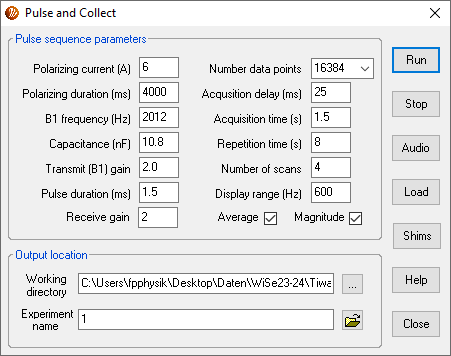
\includegraphics[width=5cm]{Live-Dokumente/Bilder/Testaufnahme-Pulse-And-Collect.PNG}
            \caption{Testaufnahme der \enquote{Pulse and Collect} Parameter.}
            \label{fig:TestPulseAndCollect}
        \end{figure}

        \paragraph*{Versuchsteil 2}
            Der Live-Plot der \texttt{Exp1} Messreihe (siehe Tabelle unten) ist gegeben durch:
            \begin{figure}[H]
                \centering
                \begin{subfigure}[b]{0.4\textwidth}
                    \centering
                    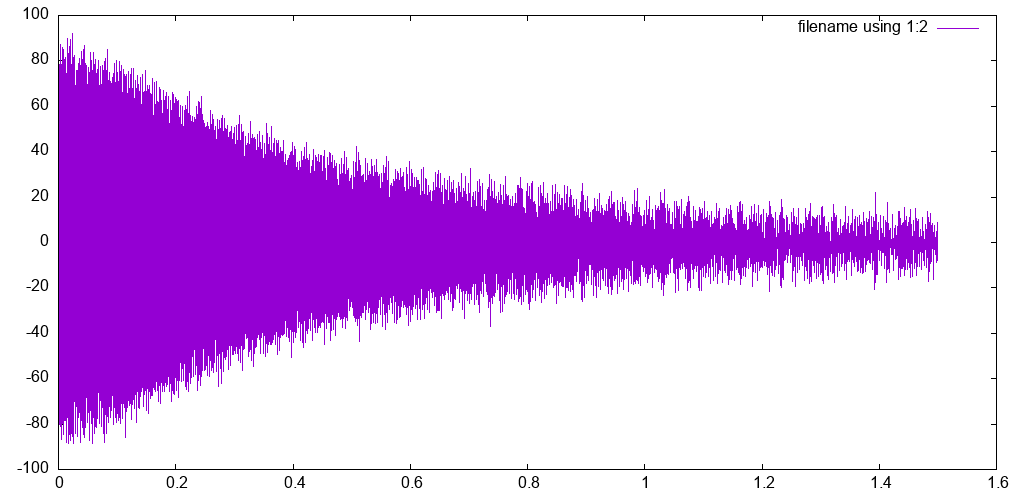
\includegraphics[width=5cm]{Live-Dokumente/Bilder/Exp1_FID.png}
                    \caption{FID.}
                \end{subfigure}
                \
                \begin{subfigure}[b]{0.4\textwidth}
                    \centering
                    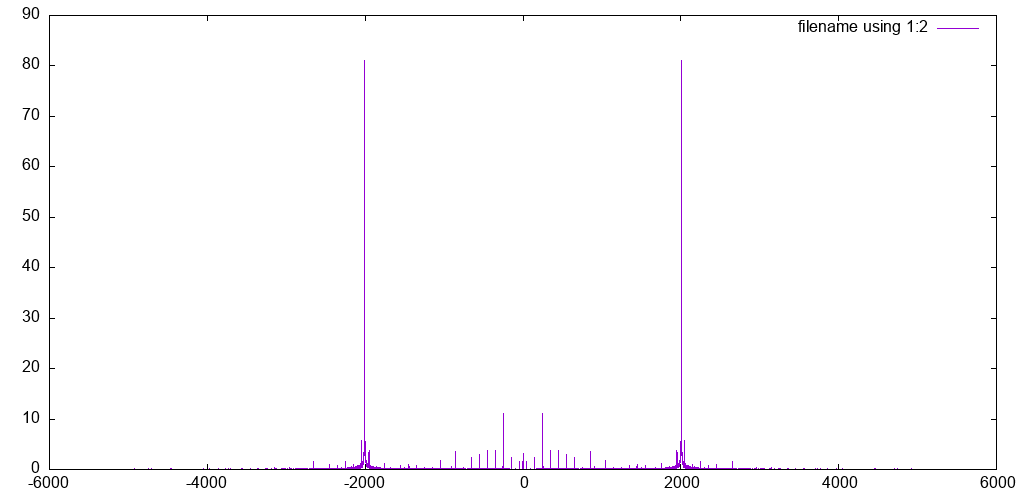
\includegraphics[width=5cm]{Live-Dokumente/Bilder/Exp1_Spectrum.png}
                    \caption{Spektrum.}
                \end{subfigure}
                \caption{Live-Plot der \texttt{Exp1} Messreihe.}
                \label{fig:LivePlotExp1}
            \end{figure}
            Wir sehen weiter Dateien mit der Erweiterung \texttt{.1d}. Um diese zu öffnen, betrachte unter \href{https://afni.nimh.nih.gov/afni/community/board/read.php?1,160269,160270}{afni.nimh.nih.gov} die Möglichkeit 
\begin{lstlisting}{language=python}
import lib_afni1D.py as LAD

my_dat = LAD.Afni1D(filename)
\end{lstlisting}


        \paragraph*{Versuchsteil 3}
            Wir sind uns unsicher, was die Aussage des Rauschens ist. 

        \paragraph*{Versuchsteil 4}

            
        \paragraph*{Versuchsteil 5}
            Wir wählen bei \enquote{Autoshim} die angegebenen Parameter. Wir erhalten dieselben Werte wie in \ref{fig:TestPulseAndCollect}, die Parameter waren also bereits optimal. \\

            Wir erhalten nicht die gewünschte Kurve. Man erkennt die Lamorfrequenz als Peak im Zentrum, vermisst allerdings die Resonanzfrequenz des LC-Schwingkreises. Die Lösung besteht darin, den Wert von \emph{aquisation delay} auf $2\si{\ms}$ zu setzen. Zusätzlich setzen wir \emph{diplay range} auf $500\si{\hertz}$. \\

            Bei der $C$ Optimierung stellen wir einen bereits optimalen Wert von $10.8\si{\nano\farad}$ fest. \\

            Bei der $B_1$ Optimierung betrachten wir den Parameter unter \emph{pulse duration}. Wir stellen $1.5\si{\seconds}$ als bereits optimiert fest, wählen nach Inspektion des FID Amplitudengraphen allerdings $1.7\si{\s}$ aus. Die finalen Werte für den Ordner \texttt{B1-Opti} sind damit:
            \marginnote{Ordnerbackup 11:00}
            \begin{figure}[H]
                \centering
                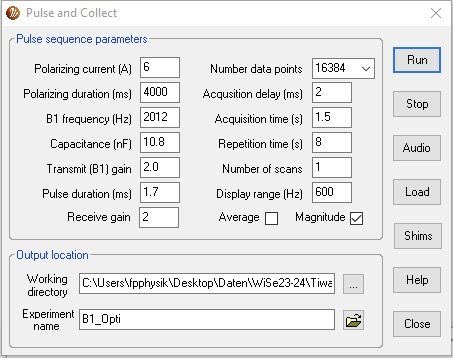
\includegraphics[width=5cm]{Live-Dokumente/Bilder/B1OptiWerte.jpeg}
                \caption{Parameter für die $B_1$ Optimierung (vor Fußnote).}
                \label{fig:B1OptiParam}
            \end{figure}
            \marginnote{Fußnote gelesen 11:15}
            Aufgrund experimenteller Einschränkungen wählen wir ein Vielfaches von $0.5\cdot (1/2012\si{\hertz})\approx 0.248\si{\s}$ aus und verwenden $1.75\si\s$.  


        \paragraph*{Versuchsteil 7}
            Wir erzeugen mit den als optimal erkannten Parametern eine FID und ihre Fouriertransformierte in \texttt{FID-Characterize1}.
            

        \paragraph*{Versuchsteil 8}
            Wir wählen das Polarisationsfeld mit $4$ nacheinanderfolgenden Scans und dem Mittelwert als Ergebnis. 
            \marginnote{Backup Ordner und Log 11:31}
            Als Ergebnisse der $10$ Schritt Messung haben wir die Relaxionszeit $T_1$ als folgenden Graphen.
            \begin{figure}[H]
                \centering
                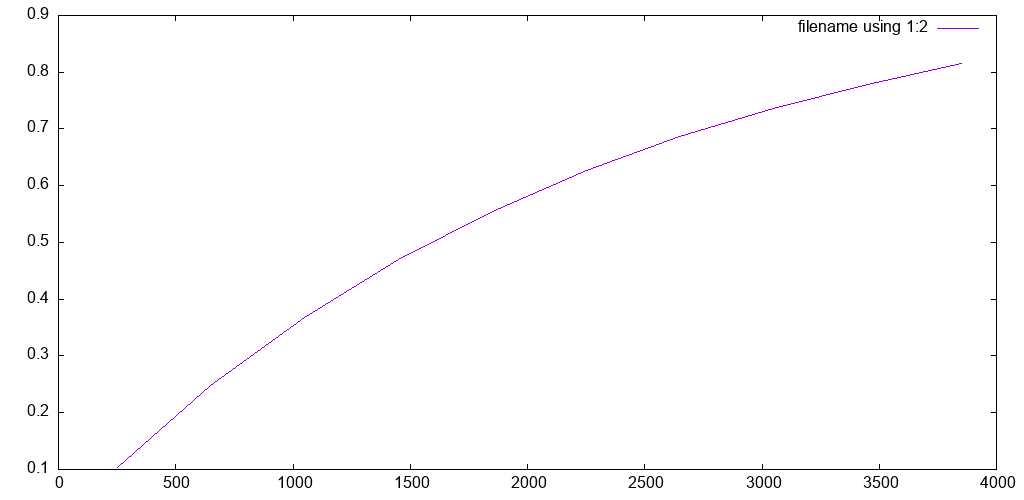
\includegraphics[width=5cm]{Live-Dokumente/Bilder/B1-10steps/T1.png}
                \caption{Amplitude $E/E_0$ über der Zeit $t$ der Polarisierungsdauer bei $10$ Schritten.}
                \label{fig:T1}
            \end{figure}
            Wir erzeugen noch eine $20$ Schritt Messung und erhalten eine Kurve mit ausgeprägterer Sättigung.
            \marginnote{Fit selber machen}
            \begin{figure}
                \centering
                \begin{subfigure}[b]{0.4\textwidth}
                    \centering
                    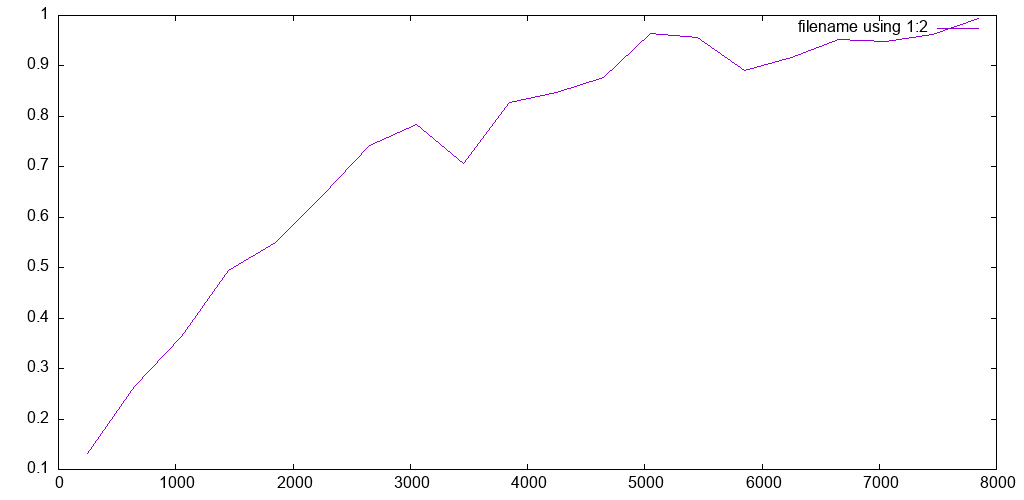
\includegraphics[width=5cm]{Live-Dokumente/Bilder/T1-20steps/T1.png}
                    \caption{Datenpunkte.}
                \end{subfigure}
                \
                \begin{subfigure}[b]{0.4\textwidth}
                    \centering
                    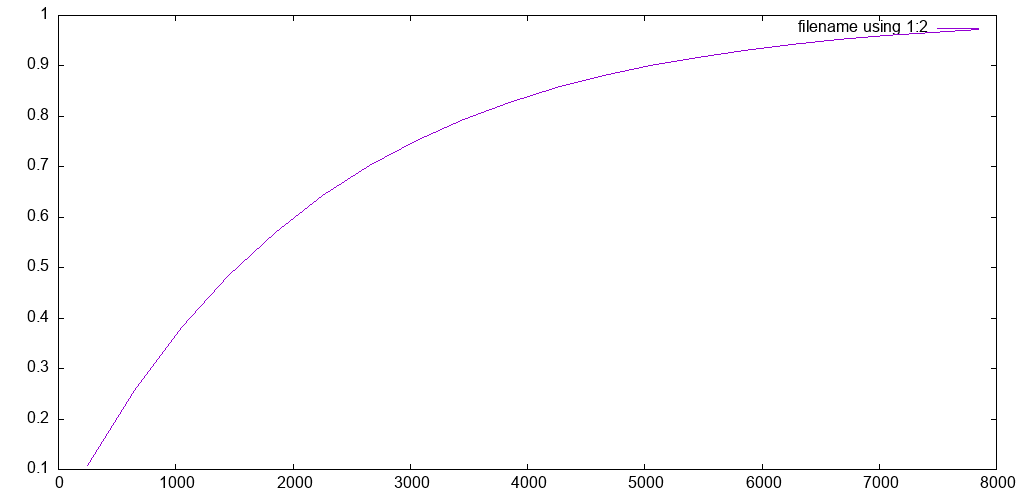
\includegraphics[width=5cm]{Live-Dokumente/Bilder/T1-20steps/T1_fit.png}
                    \caption{Curvefit.}
                \end{subfigure}
                \caption{Amplitude $E/E_0$ über der Zeit $t$ der Polarisierungsdauer bei $20$ Schritten.}
                \label{fig:T1-20steps}
            \end{figure}

        \paragraph*{Versuchsteil 9}
            \marginnote{Backup Ordner und Log 14:00}
            Wir nehmen einmal mit Idealeinstellungen auf. Dann variieren wir $x$ auf $+30$ und $-30$. Zu beiden Werten erstellen wir eine gemittelte Aufnahme (\emph{Average}) und eine ungemittelte.


        \paragraph*{Versuchsteil 10}
            Wir verwenden für die $180\si{\degree}$ puls phase den Wert $3.25\si{\ms}$. 
            \begin{itemize}
                \item Wir verwenden als \emph{echo time} den Wert $200\si{\ms}$ bzw. als \emph{dwell time} den Wert $90\si{\micro\seconds}$. $\leadsto$ \texttt{CPMG-0-0-constant2-avg}.
                \item Wir verwenden als \emph{echo time} den Wert $175\si{\ms}$ bzw. als \emph{dwell time} den Wert $90\si{\micro\seconds}$. $\leadsto$ \texttt{CPMG-0-0-constant3-avg}.
            \end{itemize}
            Das zweite Wertepaar verwenden wir für die alternierende Pulsmessung. 

        \paragraph*{Versuchsteil 11}
            Die Messung an der Wasserprobe haben wir am Anfang bereits gemacht. Wir nehmen nun das FID Spektrum mit einer \emph{polarization time} von $500\si{\ms}$ bzw. $4000\si{\ms}$. \\

            Für die $T_1$ Messung mitteln wir über $3$ Iterationen mit $15$ Schritten. Als Stoff wählen wir Mangan. \\

            Mit zunehmender Konzentration wirkt das Signal verrauschter. Wir wiederholen die Messung für $Mn$ in $200\si{\mikro\mol}$. \\
            
            \begin{figure}
                \centering
                \begin{subfigure}[b]{0.4\textwidth}
                    \centering
                    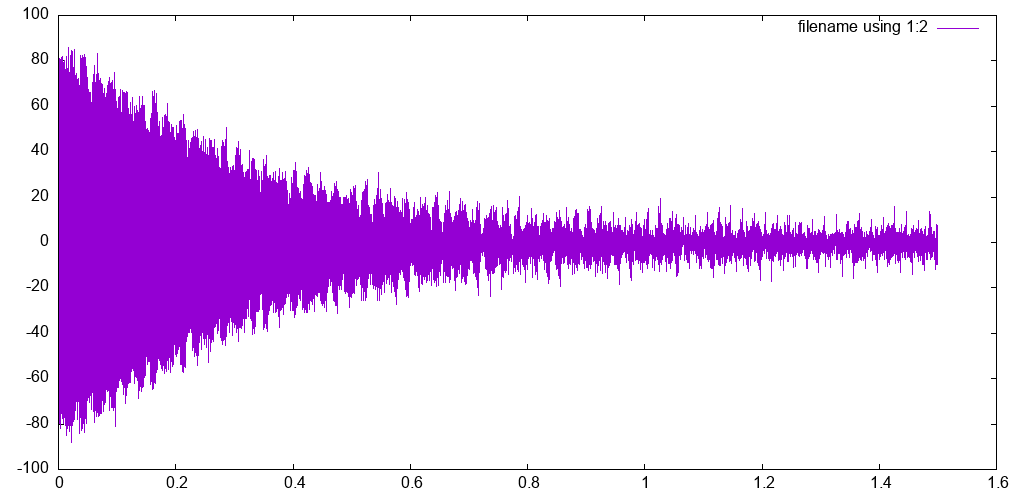
\includegraphics[width=5cm]{Live-Dokumente/Bilder/FID-11/FID_25.png}
                    \caption{FID bei $25\si{\micro\mol}$.}
                \end{subfigure}
                \
                \begin{subfigure}[b]{0.4\textwidth}
                    \centering
                    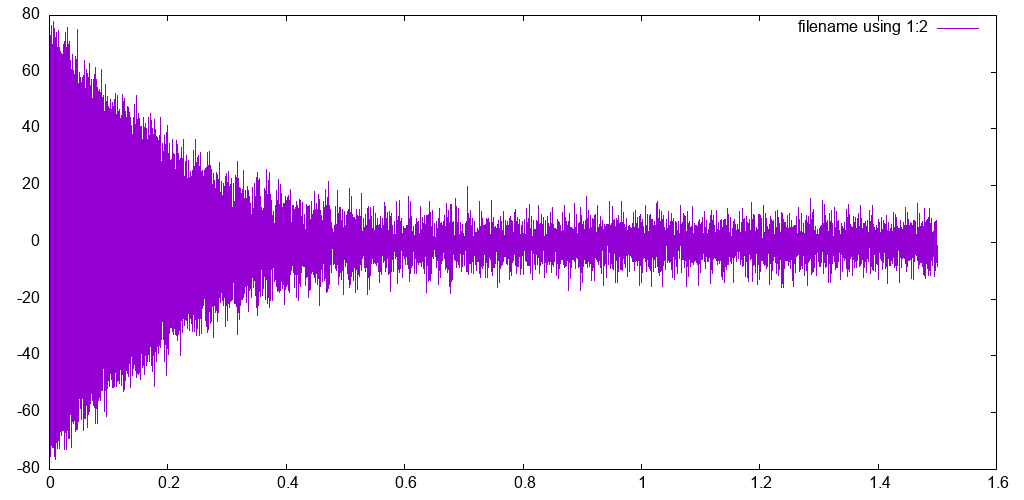
\includegraphics[width=5cm]{Live-Dokumente/Bilder/FID-11/FID_50.png}
                    \caption{FID bei $50\si{\micro\mol}$.}
                \end{subfigure}
                \
                \begin{subfigure}[b]{0.4\textwidth}
                    \centering
                    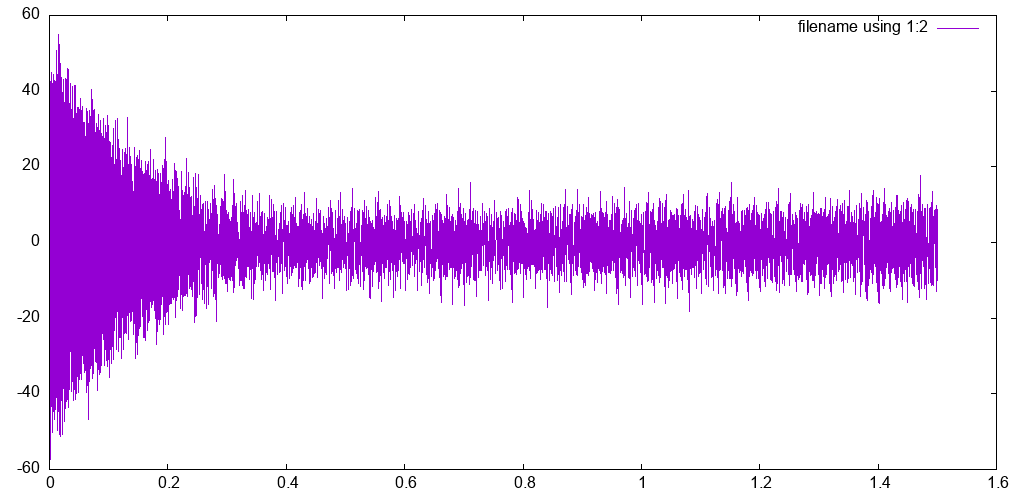
\includegraphics[width=5cm]{Live-Dokumente/Bilder/FID-11/FID_100.png}
                    \caption{FID bei $100\si{\micro\mol}$.}
                \end{subfigure}
                \
                \begin{subfigure}[b]{0.4\textwidth}
                    \centering
                    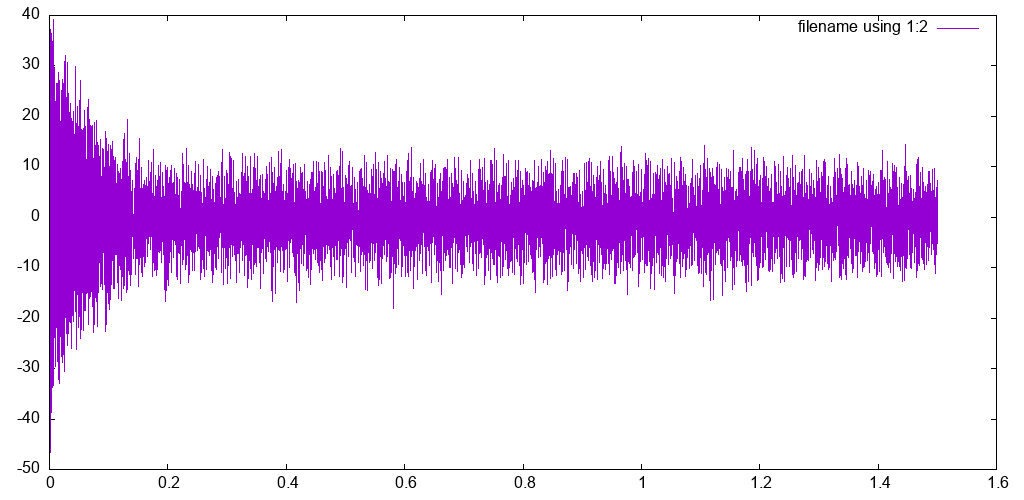
\includegraphics[width=5cm]{Live-Dokumente/Bilder/FID-11/FID_200.png}
                    \caption{FID bei $200\si{\micro\mol}$.}
                \end{subfigure}
                \caption{FID bei verschiedenen Konzentrationen von Manganionen $Mn^{2+}$ in Wasser.}
            \end{figure}


        \paragraph*{Versuchsteil 12}
            Vermessung des Phantoms. Gesamtdurchmesser ist $7.5(1)\si{\cm}$. Der Durchmesser der inneren Zylinder ist $3.0(1)\si{\cm}$ im Durchmesser, der Abstand der Röhrenmitten beträgt $3.5(1)\si{\cm}$. Die inneren Zylinder haben eine Höhe von $13.0(2)\si{\cm}$.

        \paragraph*{Dateinamen}

        \begin{table}[H]
            \centering
            \begin{tabular}{p{4cm}|c|p{6cm}}
                \textbf{Dateiname} & \textbf{Nutzbarkeit} & \textbf{Bedeutung} \\
                \hline\hline
                \texttt{Exp1} & & \\
                \texttt{Exp2} & & \\
                \hline
                \texttt{AutoShim1} & x & Testlauf des \emph{auto-shimming} \\
                \texttt{AutoShim2} & & \\
                \hline
                \texttt{Explore-FID1} & & Testaufnahme unter Varrierung von \emph{recieve gain} \\
                \texttt{Explore-FID2} & & \\
                \texttt{Explore-FID3} & & \\
                \hline
                \texttt{C-Opti} & x & Wert $10.8$ war bereits optimiert. \\
                \hline
                \texttt{B1DurationFast} & & \\
                \texttt{B1Opti} & & \\
                \hline
                \texttt{FID-Characterize1} & x & Optimale Einstellungen mit \emph{pulse duration} auf $25\si{\ms}$\\
                \texttt{FID-Characterize2} & & \\
                \hline
                \texttt{T1-Bp-10steps} & & Spin-Gitter-Relaxion im Polarisationsfeld \\
                \texttt{T1-Bp-20steps} & & \\
                \hline
                \texttt{Echo-optimal-}\texttt{positive-multi-average} & & \\
            \end{tabular}
        \end{table}
\end{document}